%
% main.tex -- Paper zum Thema <elliptisch>
%
% (c) 2020 Autor, OST Ostschweizer Fachhochschule
%
% !TEX root = ../../buch.tex
% !TEX encoding = UTF-8
%
\chapter{Elliptische Integrale}\label{chapter:elliptisch}
\kopflinks{Elliptische Integrale}
\begin{refsection}
\chapterauthor{Baris Catan}

\index{Baris Catan}%
\index{Catan, Baris}%

\noindent
Der Umfang einer Ellipse führt auf ein Integral, das keine
elementare Stammfunktion besitzt. 
Dass das so ist, kann die Analysis nicht zeigen, denn sie liefert
nur Existenzaussagen.
Der Nachweis gelingt erst mit algebraischen Methoden.
Mit dem Satz von Liouville und dem Risch-Algorithmus, die im
Kapitel~\ref{chapter:intalg} dargestellt wurden, setzen wir
der elementaren Integration eine scharfe Grenze und zeigen, dass
das Ellipsenintegral diese Grenze überschreitet.
In diesem Kapitel wird zuerst diese Grenze bestimmt, dann werden
die elliptischen Integrale eingeführt und umgekehrt.
Gerade diese Umkehrung ist der Durchbruch des Themas, sie liefert
die jacobischen elliptischen Funktionen, mit denen sich am Schluss
Anwendungen wie das Pendel, die Lemniskate und das rotierende
Springseil exakt behandeln lassen.

%
% einleitung.tex -- Einleitung und Motivation
%
% (c) 2026 Baris Catan, OST Ostschweizer Fachhochschule
%
% !TEX root = ../../buch.tex
% !TEX encoding = UTF-8
%
\section{Eine harmlose Frage
\label{elliptisch:section:einleitung}}
\kopfrechts{Eine harmlose Frage}

Wir beginnen dieses Kapitel mit einer Frage, die einfacher klingt,
als sie ist.
Wie lang ist der Umfang einer Ellipse?
Für den Kreis mit Radius $r$ genügt die Parametrisierung
$(x,y) = (r\cos t,\, r\sin t)$.
Wegen $\sin^2 t + \cos^2 t = 1$ fällt die Wurzel im Bogenelement weg
und es bleibt
\begin{equation}
U
=
\int_0^{2\pi} \sqrt{\dot x^2 + \dot y^2}\,dt
=
\int_0^{2\pi} \sqrt{r^2\sin^2 t + r^2\cos^2 t}\,dt
=
\int_0^{2\pi} r\,dt
=
2\pi r.
\label{elliptisch:equation:kreisumfang}
\end{equation}

Dieselbe Rechnung führen wir nun für die Ellipse mit den Halbachsen
$a \ge b$ durch, parametrisiert durch
$(x,y) = (a\cos t,\, b\sin t)$
(siehe Abbildung~\ref{fig:elliptisch:ellipse}).
\begin{figure}
	\centering
	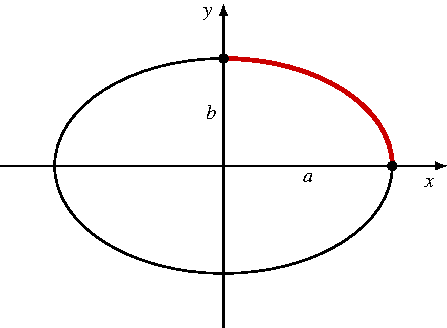
\includegraphics[width=0.6\textwidth]{papers/elliptisch/images/ellipse.pdf}
	\caption{Die Ellipse mit den Halbachsen $a$ und $b$.
	Hervorgehoben ist der Bogen im ersten Quadranten, der volle
	Umfang ist aus Symmetriegründen das Vierfache.}
	\label{fig:elliptisch:ellipse}
\end{figure}

Das Bogenelement ist
\begin{equation}
ds
=
\sqrt{\dot x^2 + \dot y^2}\,dt
=
\sqrt{a^2\sin^2 t + b^2\cos^2 t}\,dt
=
a\,\sqrt{1 - k^2\cos^2 t}\,dt,
\qquad
k^2 = \frac{a^2-b^2}{a^2},
\label{elliptisch:equation:bogenelement}
\end{equation}
wobei $k$ die numerische Exzentrizität ist
\cite{elliptisch:mueller-spezielle}, später auch Modul
genannt.
\index{Ellipse}%
\index{Exzentrizitat@Exzentrizität}%
Bemerkenswert ist, dass diesmal die Wurzel nicht verschwindet.
Wegen der Symmetrie der Ellipse genügt der erste Quadrant, der
volle Umfang
\begin{equation}
U
=
4a \int_0^{\pi/2} \sqrt{1 - k^2\cos^2 t}\,dt
\label{elliptisch:equation:umfangcos}
\end{equation}
ist das Vierfache davon.
Die Substitution $t \mapsto \frac{\pi}{2} - t$ bildet das Intervall
$[0, \pi/2]$ auf sich ab und vertauscht $\cos^2$ mit $\sin^2$.
Somit erhalten wir
\begin{equation}
U
=
4a \int_0^{\pi/2} \sqrt{1 - k^2\sin^2 t}\,dt.
\label{elliptisch:equation:umfang}
\end{equation}
Für den Kreis ist $a = b = r$, also $k = 0$, eingesetzt in
\eqref{elliptisch:equation:umfang} liefert
$U = 4a \cdot \frac{\pi}{2} = 2\pi r$, wie erwartet.
Wie sich herausstellen wird, hat das Integral
\eqref{elliptisch:equation:umfang} jedoch keine elementare Stammfunktion.

\subsection{Existenz und Darstellbarkeit}
\begin{satz}[Hauptsatz der Differential- und Integralrechnung]
Ist $f$ stetig, dann ist $F(x) = \int_a^x f(t)\,dt$
differenzierbar mit $F' = f$, insbesondere besitzt $f$ eine
Stammfunktion.
\end{satz}
Über die Existenz einer Stammfunktion muss man also nie streiten.
Ganz anders sieht es mit der \emph{Darstellbarkeit} aus.
Ob sich $F$ als endliche Formel aus Polynomen, Wurzeln, $\exp$,
$\log$ und den trigonometrischen Funktionen schreiben lässt,
ist eine völlig andere Frage.
Existenz heisst nicht Darstellbarkeit.
Funktionen, die aus Polynomen, Wurzeln, $\exp$, $\log$ und den
trigonometrischen Funktionen zusammengesetzt sind, heissen
\emph{elementar}, der Begriff wird weiter unten präzisiert und ist
ausführlich in Abschnitt~\ref{buch:intalg:section:elementar}
behandelt.
Drei Beispiele zeigen, wie weit Existenz und Darstellbarkeit
auseinanderliegen können.

Integranden mit der Wurzel aus einem quadratischen Polynom sind
stets elementar integrierbar, zum Beispiel
\begin{equation}
\int \sqrt{x^2+1}\,dx
=
\frac{1}{2}\left(x\sqrt{x^2+1} + \operatorname{arsinh} x\right),
\label{elliptisch:equation:wurzelstandard}
\end{equation}
dessen Stammfunktion handhabbar ist, um damit weiterzurechnen.
Abschnitt~\ref{buch:intalg:section:wurzel} zeigt, dass dies für
jedes quadratische Polynom unter der Wurzel gelingt.

Schon der Integrand $\sqrt{\tan x}$ zeigt jedoch, dass aus
elementar lösbar nicht brauchbar folgt.
Die Substitution $u = \sqrt{\tan x}$ macht den Integranden
rational,
\begin{equation}
\int \sqrt{\tan x}\,dx
=
\int \frac{2u^2}{1+u^4}\,du,
\label{elliptisch:equation:tanxrational}
\end{equation}
und die Partialbruchzerlegung über die Faktorisierung
$1+u^4 = (u^2-\sqrt{2}u+1)(u^2+\sqrt{2}u+1)$
garantiert eine elementare Stammfunktion.
Ein Computeralgebrasystem liefert sie auch, nämlich
\begin{equation}
\frac{\sqrt{2}}{4}
\log\frac{\tan x-\sqrt{2}\sqrt{\tan x}+1}
        {\tan x+\sqrt{2}\sqrt{\tan x}+1}
+
\frac{\sqrt{2}}{2}\arctan\left(\sqrt{2}\sqrt{\tan x}-1\right)
+
\frac{\sqrt{2}}{2}\arctan\left(\sqrt{2}\sqrt{\tan x}+1\right).
\label{elliptisch:equation:tanxmonster}
\end{equation}
Der Ausdruck ist so unhandlich, dass er für praktische Zwecke
kaum etwas nützt.

Beim dritten Beispiel versagt die elementare Integration
vollständig.
Für
\begin{equation}
\int e^{-x^2}\,dx
\label{elliptisch:equation:expx2}
\end{equation}
lässt sich beweisen, dass keine elementare Stammfunktion existiert,
der Beweis wird in Abschnitt~\ref{buch:intalg:section:risch}
geführt.
An dieser Stelle ist die Konsequenz wichtiger als der Beweis.
Wenn keine elementare Stammfunktion existiert, bleibt nur, dem
Integral einen Namen zu geben und es selbst zur Funktion zu
erklären.
Für dieses Integral ist das geschehen, die Fehlerfunktion
\begin{equation}
\operatorname{erf}(x)
=
\frac{2}{\sqrt{\pi}} \int_0^x e^{-t^2}\,dt
\label{elliptisch:equation:erfx}
\end{equation}
ist nichts anderes als die Stammfunktion von $e^{-x^2}$ in
normierter Form.
\index{Fehlerfunktion}%
Dasselbe Prinzip steckt hinter der Definition
$\log x = \int_1^x \frac{dt}{t}$,
und genau derselbe Schritt wird in diesem Kapitel mit den
elliptischen Integralen vollzogen.
Was nicht elementar integrierbar ist, wird zur neuen Funktion.
Die Frage, welche Integranden eine elementare Stammfunktion
besitzen, ist damit keine Frage der Analysis, sondern der Algebra.

\subsection{Elementare Funktionen}
Der Begriff der elementaren Funktion, den wir bisher nur
umgangssprachlich verwendet haben, lässt sich algebraisch fassen.
Ausgangspunkt ist der Körper $F_0 = \mathbb{Q}(x)$ der rationalen
Funktionen zusammen mit der gewöhnlichen Ableitung.
In jedem weiteren Schritt kommt eine einzelne neue Funktion
$\vartheta$ dazu, die über dem bisherigen Körper algebraisch ist oder
zu einem $v$ des bisherigen Körpers die Gleichung $\vartheta' = v'/v$
erfüllt, also ein Logarithmus ist, oder die Gleichung
$\vartheta'/\vartheta = v'$, also eine Exponentialfunktion
(siehe Abschnitt~\ref{buch:intalg:section:elementar}).
So entsteht ein \emph{Turm}
\begin{equation}
F_0 \subset F_1 \subset \dots \subset F_N,
\qquad
F_i = F_{i-1}(\vartheta_i),
\label{elliptisch:equation:koerperturm}
\end{equation}
von Körpererweiterungen.
Jeder Körper $F_i$ darin ist eine Erweiterung seines Vorgängers um
genau eine neue Funktion $\vartheta_i$.
Eine Funktion heisst \emph{elementar}, wenn sie sich in endlich
vielen solchen Schritten aufbauen lässt
(Abbildung~\ref{fig:elliptisch:koerperturm}).
\index{elementare Funktion}%
\index{Korperturm@Körperturm}%
\begin{figure}
	\centering
	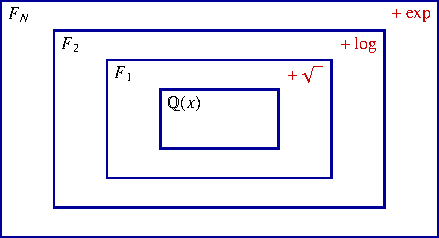
\includegraphics[width=0.7\textwidth]{papers/elliptisch/images/koerperturm.pdf}
	\caption{Eine elementare Funktion liegt in einem endlichen Turm
	von Körpererweiterungen, ausgehend von den rationalen Funktionen
	$\mathbb{Q}(x)$.
	In jedem Schritt kommt eine Wurzel, ein Logarithmus oder eine
	Exponentialfunktion dazu.}
	\label{fig:elliptisch:koerperturm}
\end{figure}

Die Sinus- und Kosinusfunktion fehlen in dieser Aufzählung nicht,
sie stecken über $\sin x = (e^{ix}-e^{-ix})/2i$ bereits in den
exponentiellen Schritten.
Die Wurzel $\sqrt{p(x)}$ ist ein algebraischer Schritt, denn sie
erfüllt die Gleichung $\vartheta^2 - p(x) = 0$ über
$\mathbb{Q}(x)$.
Alles, was sich als endliche Formel hinschreiben lässt, ist damit
erfasst.

\subsection{Der Satz von Liouville}
Ableiten führt aus einem solchen Turm nie heraus.
Liegt $f$ in einem der Körper $F_i$, dann liegt auch $f'$ wieder in
$F_i$, denn Summen-, Produkt- und Kettenregel erzeugen nur
Ausdrücke in bereits vorhandenen Elementen.
Beim Integrieren gilt das nicht, schon $\int dx/x = \log x$ verlässt
den Körper $\mathbb{Q}(x)$.
Die Frage ist also, wie weit man im Turm hinaufsteigen muss, um eine
Stammfunktion zu erreichen.
Liouville hat sie ab 1833 beantwortet
\cite{elliptisch:wiki-liouville}, und die
Antwort fällt enger aus, als man erwarten würde.
\index{Liouville, Satz von}%
\begin{satz}[Prinzip von Liouville]
\label{elliptisch:satz:liouville}
Sei $F$ ein Funktionenkörper mit Konstantenkörper $C$ und $f \in F$.
Besitzt $f$ eine Stammfunktion in einer elementaren Erweiterung von
$F$ mit demselben Konstantenkörper, dann gibt es Elemente
$v_0, v_1, \dots, v_n \in F$ und Konstanten
$c_1, \dots, c_n \in C$ mit
\begin{equation}
\int f\,dx
=
v_0 + \sum_{i=1}^n c_i \log v_i.
\label{elliptisch:equation:liouville}
\end{equation}
\end{satz}
Der Beweis wird in Abschnitt~\ref{buch:intalg:section:liouville}
geführt.
An dieser Stelle interessiert uns, was die Aussage leistet.

Ohne diesen Satz müsste die Stammfunktion in einer beliebig grossen
elementaren Erweiterung von $F$ gesucht werden, mit beliebig vielen
neuen Wurzeln, Exponentialfunktionen und ineinander geschachtelten
Logarithmen.
Somit ist die Art, wie die Stammfunktion aussieht, relativ starr.
Die Bausteine $v_0$ und $v_i$ liegen bereits in $F$, hinzu kommen
einzig die Logarithmen $\log v_i$, und deren Vorfaktoren $c_i$ sind
Konstanten.
Eine Exponentialfunktion, die im Integranden nicht vorkommt, kann in
der Stammfunktion also gar nicht auftauchen, und ein Logarithmus
eines Logarithmus ebenso wenig.
Der Turm über $F$, in dem die Stammfunktion zu suchen ist, hat damit
nur noch eine einzige Etage.

Zum Rechnen eignet sich die abgeleitete Fassung
\begin{equation}
f
=
v_0' + \sum_{i=1}^n c_i \frac{v_i'}{v_i}
\label{elliptisch:equation:liouvilleableitung}
\end{equation}
besser, denn sie enthält kein Integral mehr und ist eine Gleichung
innerhalb von $F$.
Aus der Existenzfrage wird damit eine Rechnung.
Man setzt die Form \eqref{elliptisch:equation:liouvilleableitung} mit
unbekannten $v_i$ und $c_i$ an und vergleicht Koeffizienten.
Geht die Rechnung auf, ist die Stammfunktion gefunden.
Führt sie auf einen Widerspruch, so ist bewiesen, dass keine
elementare Stammfunktion existiert.
Auf diesem Weg wird in
Abschnitt~\ref{buch:intalg:section:risch} gezeigt, dass $e^{-x^2}$
keine elementare Stammfunktion besitzt.
Risch hat das Verfahren in den Sechzigerjahren zu einem Algorithmus
ausgebaut \cite{elliptisch:risch}, der die Frage in endlich vielen
Schritten entscheidet.
Abschnitt~\ref{buch:intalg:section:risch} stellt ihn ausführlich dar.
Dieser Risch-Algorithmus steckt heute im Kern der
Integrationsroutinen von Computeralgebrasystemen.
\index{Risch-Algorithmus}%

%
% grenze.tex -- Die Grenze der elementaren Integration
%
% (c) 2026 Baris Catan, OST Ostschweizer Fachhochschule
%
% !TEX root = ../../buch.tex
% !TEX encoding = UTF-8
%
\section{Die Grenze der elementaren Integration
\label{elliptisch:section:grenze}}
\kopfrechts{Die Grenze}

In der Einleitung haben wir behauptet, das Integral
\eqref{elliptisch:equation:umfang} habe keine elementare
Stammfunktion.
In diesem Abschnitt wollen wir genauer untersuchen, wo die Grenze
zwischen elementar und nicht elementar verläuft.
Es geht dabei durchgehend um Integranden der Form
$R\bigl(x,\sqrt{p(x)}\bigr)$, also um rationale Funktionen in $x$
und in der Wurzel aus einem Polynom $p(x)$.

\subsection{Der quadratische Fall
\label{elliptisch:subsection:quadratisch}}
\index{Euler-Substitution}%
Für ein Polynom vom Grad höchstens $2$ ist die Lage vollständig
geklärt.
Wir schreiben
\begin{equation}
\vartheta = \sqrt{ax^2 + bx + c}
\label{elliptisch:equation:theta}
\end{equation}
und betrachten Integranden, die rational in $x$ und $\vartheta$
sind.
Mithilfe der Euler-Substitution $\vartheta = \sqrt{a}\,x + t$ (für
$a > 0$) lässt sich $x$ als rationale Funktion von $t$ schreiben.
Quadrieren der Substitutionsgleichung und Vergleichen mit
$\vartheta^2 = ax^2 + bx + c$ ergibt
\begin{equation}
x
=
\frac{c - t^2}{2\sqrt{a}\,t - b},
\label{elliptisch:equation:eulersubst}
\end{equation}
und damit werden auch $dx$ und $\vartheta$ rational in $t$
(Kapitel~\ref{chapter:ratint}).
Der Integrand wird dadurch zu einer rationalen Funktion von $t$
allein, und rationale Funktionen sind stets elementar integrierbar.
Die Partialbruchzerlegung erzeugt nur Bausteine, deren
Stammfunktionen Logarithmen, Potenzen und Arkustangens sind.
Ein Resultat dieser Rechnung ist
\begin{equation}
\int \frac{dx}{\vartheta}
=
\frac{1}{\sqrt{a}}\,
\log\bigl(2ax + b + 2\sqrt{a}\,\vartheta\bigr),
\label{elliptisch:equation:quadratisch}
\end{equation}
zu finden in
Abschnitt~\ref{buch:intalg:wurzel:subsection:stammfunktiontheta}.
Die Gestalt der rechten Seite ist typisch für diesen Fall.
Sie besteht aus einem konstanten Vorfaktor und dem Logarithmus
eines Elements des Funktionenkörpers.
Das ist genau die Form \eqref{elliptisch:equation:liouville}, die der Satz 
von Liouville für eine elementare
Stammfunktion verlangt, hier mit $v_0 = 0$ und einem einzigen
Logarithmusterm.
Steht unter der Wurzel ein Polynom vom Grad $\le 2$, so ist das
Integral immer elementar lösbar.

\subsection{Definition des elliptischen Integrals}
Ab Grad $3$ versagt dieses Verfahren, der Grund dafür wird in
Abschnitt~\ref{elliptisch:subsection:wurzelbleibt} deutlicher.
\begin{definition}
\index{elliptisches Integral}%
Ein \emph{elliptisches Integral} ist ein Integral der Form
\begin{equation}
\int R\bigl(x, \sqrt{p(x)}\bigr)\,dx,
\label{elliptisch:equation:definition}
\end{equation}
wobei $R$ eine rationale Funktion in zwei Variablen ist und $p$ ein
Polynom vom Grad $3$ oder $4$ ohne mehrfache Nullstellen.
\end{definition}
Die Bedingung an die Nullstellen ist wesentlich.
Hätte $p$ eine doppelte Nullstelle, also
$p(x) = (x-\alpha)^2 q(x)$, dann liesse sich der Faktor aus der
Wurzel ziehen, $\sqrt{p(x)} = |x-\alpha|\sqrt{q(x)}$, und der
effektive Grad sänke auf höchstens $2$.
Wir wären damit wieder im quadratischen Fall des vorangegangenen
Abschnitts.
Die Grade $3$ und $4$ stehen in der Definition zusammen, weil sie
dieselbe Schwierigkeitsklasse bilden.
Ist $\deg p = 4$ und $\alpha$ eine Nullstelle von $p$, so schreiben
wir $p(x) = (x-\alpha)q(x)$ mit $\deg q = 3$ und substituieren
$x = \alpha + 1/u$.
Wegen $dx = -du/u^2$ und
\begin{equation}
p\biggl(\alpha+\frac{1}{u}\biggr)
=
\frac{1}{u}\,q\biggl(\alpha+\frac{1}{u}\biggr)
=
\frac{Q(u)}{u^4},
\qquad
Q(u) = u^3\,q\biggl(\alpha+\frac{1}{u}\biggr),
\label{elliptisch:equation:gradreduktion}
\end{equation}
mit einem Polynom $Q$ vom Grad höchstens $3$ kürzt sich das $u^2$
aus der Wurzel gegen dasjenige in $dx$, und es bleibt
\begin{equation}
\frac{dx}{\sqrt{\smash[b]{\underbrace{p(x)}_{\text{Grad } 4}}}}
=
-\frac{du}{\sqrt{\smash[b]{\underbrace{Q(u)}_{\text{Grad } 3}}}}.
\label{elliptisch:equation:gradreduziert}
\end{equation}
\vspace{0.6ex}

\noindent
Aus dem Grad $4$ ist damit Grad $3$ geworden, und dieselbe
Substitution führt umgekehrt von Grad $3$ auf Grad $4$.
Polynome vom Grad $5$ und mehr führen auf die
\emph{hyperelliptischen} Integrale, die wir hier nicht behandeln.
\index{hyperelliptisches Integral}%
Abbildung~\ref{fig:elliptisch:gradskala} fasst diese Einteilung
zusammen.
\begin{figure}
	\centering
	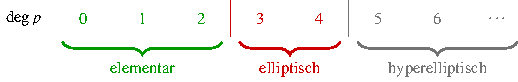
\includegraphics[width=0.9\textwidth]{papers/elliptisch/images/gradskala.pdf}
	\caption{Der Grad des Polynoms $p$ unter der Wurzel entscheidet
	über die Lösbarkeit.
	Bis Grad $2$ ist das Integral elementar, bei den Graden $3$ und
	$4$ elliptisch, ab Grad $5$ hyperelliptisch.}
	\label{fig:elliptisch:gradskala}
\end{figure}
%
Den Namen haben die elliptischen Integrale vom geometrischen
Problem, zu dem wir jetzt zurückkehren, nämlich der Bogenlänge
der Ellipse.

\subsection{Das Ellipsenumfangsintegral}
In der Einleitung haben wir den Umfang der Ellipse auf das Integral
\eqref{elliptisch:equation:umfang} gebracht.
Warum es in die Definition \eqref{elliptisch:equation:definition}
fällt, sehen wir nach einer weiteren Substitution.
Das Kriterium verlangt eine rationale Variable, wir setzen daher
$x = \sin t$ mit $dt = dx/\sqrt{1-x^2}$ und erhalten mit den neuen
Grenzen $0$ und $1$
\begin{equation}
U
=
4a \int_0^1 \frac{\sqrt{1-k^2x^2}}{\sqrt{1-x^2}}\,dx
=
4a \int_0^1
\frac{\sqrt{(1-x^2)(1-k^2x^2)}}{1-x^2}\,dx.
\label{elliptisch:equation:umfangsubstituiert}
\end{equation}
Unter der Wurzel steht mit
\begin{equation}
p(x)
=
(1-x^2)(1-k^2x^2)
=
k^2x^4 - (1+k^2)x^2 + 1
\label{elliptisch:equation:gradvier}
\end{equation}
ein Polynom vom Grad $4$ in $x$, das für $0 < k < 1$ keine
mehrfachen Nullstellen hat.
Somit erfüllt das Ellipsenumfangsintegral genau die Definition
\eqref{elliptisch:equation:definition} und ist ein elliptisches
Integral.
Zu beachten ist noch, dass der Integrand in
\eqref{elliptisch:equation:umfangsubstituiert} bei $x = 1$ eine
Singularität hat.
Das Integral ist dort uneigentlich, aber konvergent, da der Zähler
wie $\sqrt{1-x}$ verschwindet.

\subsection{Warum die Wurzel bleibt
\label{elliptisch:subsection:wurzelbleibt}}

Mit der Einordnung als elliptisches Integral ist noch nichts über
die Lösbarkeit gesagt.
Die Definition \eqref{elliptisch:equation:definition} beschreibt eine
Bauform, keine Unmöglichkeit.
Das sieht man an
\begin{equation}
\int \frac{p'(x)}{2\sqrt{p(x)}}\,dx
=
\sqrt{p(x)},
\label{elliptisch:equation:zufallelementar}
\end{equation}
denn der Integrand ist rational in $x$ und $\sqrt{p(x)}$, das
Polynom $p$ darf Grad $4$ haben und quadratfrei sein, und trotzdem
ist die Stammfunktion elementar.
Die Frage nach der elementaren Lösbarkeit muss also für jedes
Integral einzeln gestellt werden.

Warum sie im quadratischen Fall stets zu bejahen ist, liegt tiefer
als in der Rechnung von
Abschnitt~\ref{elliptisch:subsection:quadratisch}.
Die Gleichung $\vartheta^2 = ax^2+bx+c$ beschreibt einen
Kegelschnitt, und die Euler-Substitution
\eqref{elliptisch:equation:eulersubst} ist seine rationale
Parametrisierung.
Sie drückt $x$ und $\vartheta$ rational durch $t$ aus, und umgekehrt
ist $t = \vartheta - \sqrt{a}\,x$ rational in $x$ und $\vartheta$.
Genau diese beidseitig rationale Zuordnung überträgt den
Integranden in eine rationale Funktion von $t$.
Für $\deg p \in \{3,4\}$ ist die Kurve $y^2 = p(x)$ dagegen eine
elliptische Kurve, und eine solche besitzt keine rationale
Parametrisierung \cite{elliptisch:geddes}.
\index{elliptische Kurve}%
Es gibt also keine Substitution, die den Integranden rational macht.
Der Weg des quadratischen Falls ist damit versperrt, und die Wurzel
bleibt stehen.

Dass kein anderer Weg zum Ziel führt, folgt daraus noch nicht.
Der Satz von Liouville
\eqref{elliptisch:equation:liouville} liefert an dieser Stelle eine
notwendige Bedingung.
Er sagt, welche Gestalt eine elementare Stammfunktion haben müsste,
und der Nachweis der Nichtexistenz besteht darin, diese Gestalt zu
widerlegen.
Für algebraische Erweiterungen ist das erheblich aufwendiger als für
logarithmische und exponentielle.
Polynome lassen sich dort nicht mehr eindeutig faktorisieren, der
euklidische Algorithmus fällt weg, und an seine Stelle treten
Divisoren aus der algebraischen Geometrie
\cite{elliptisch:geddes}.
Abschnitt~\ref{buch:intalg:risch:algebraisch} beschreibt, was dazu
nötig wäre, und verzichtet aus demselben Grund auf die Ausführung.
Wir übernehmen das Resultat.
%
% memeFIG.tex
%
% (c) 2026 Prof Dr Andreas Müller
%
\begin{figure}
\centering
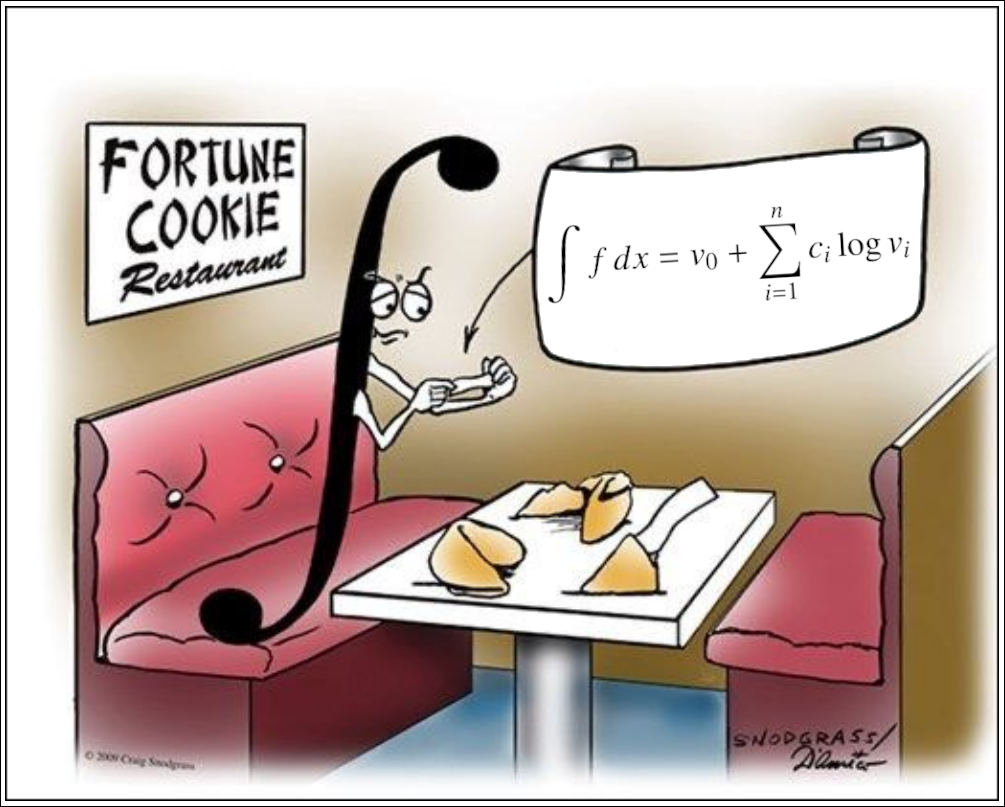
\includegraphics[width=\textwidth]{papers/elliptisch/images/meme2.png}
\caption{Das Prinzip von Liouville (Satz~\ref{elliptisch:satz:liouville})
charakterisiert die Funktionen, die eine elementare Stammfunktionen haben.
Dieses Meme stellt es als ein Fortune Cookie dar, welches dem Integral
vorhersagt, ob es mit einem Integranden Glück haben wird wird.
\label{elliptisch:meme}}
\end{figure}


\begin{satz}
\label{elliptisch:satz:nichtelementar}
Für $0 < k < 1$ besitzt keines der beiden Integrale
\begin{equation}
\int \frac{dx}{\sqrt{(1-x^2)(1-k^2x^2)}}
\qquad\text{und}\qquad
\int \frac{\sqrt{1-k^2x^2}}{\sqrt{1-x^2}}\,dx
\label{elliptisch:equation:nichtelementar}
\end{equation}
eine elementare Stammfunktion.
\end{satz}
Eine Beweisskizze und die Verweise auf die Spezialliteratur geben
Geddes, Czapor und Labahn \cite{elliptisch:geddes}.
Das zweite Integral in \eqref{elliptisch:equation:nichtelementar} ist
bis auf den Faktor $4a$ genau der Umfang der Ellipse aus
\eqref{elliptisch:equation:umfangsubstituiert}.
Die Frage vom Anfang des Kapitels ist damit beantwortet, wenn auch
negativ.
Eine elementare Formel für den Ellipsenumfang gibt es nicht, und die
Suche danach war von Beginn an aussichtslos.
Was bleibt, ist der Schritt, den wir schon bei der Fehlerfunktion
gesehen haben.
Das Integral bekommt einen Namen und wird selbst zur Funktion.

%
% funktionen.tex -- Neue Funktionen: elliptische Integrale und Funktionen
%
% (c) 2026 Baris Catan, OST Ostschweizer Fachhochschule
%
% !TEX root = ../../buch.tex
% !TEX encoding = UTF-8
%
\section{Neue Funktionen
\label{elliptisch:section:funktionen}}
\kopfrechts{Neue Funktionen}

Im vorherigen Abschnitt ist das Umfangsintegral
\eqref{elliptisch:equation:umfang} als elliptisches Integral ohne
elementare Stammfunktion eingeordnet worden.
Die Definition \eqref{elliptisch:equation:definition} lässt für die
rationale Funktion $R$ und das Polynom $p$ unendlich viele
Möglichkeiten zu, und für jede davon eine eigene Funktion
einzuführen wäre unpraktisch und, wie sich zeigen wird, auch gar
nicht nötig.

\subsection{Der Reduktionssatz}
Die elliptischen Integrale bilden zwar eine unübersehbare Menge,
aber sie unterscheiden sich nur um elementare Anteile, und was
davon übrig bleibt, sind drei feste Integrale.
\begin{satz}[Reduktionssatz]
\label{elliptisch:satz:reduktion}
Jedes elliptische Integral lässt sich als Summe elementarer
Funktionen und der drei Integrale
\begin{equation}
\int \frac{dt}{\sqrt{p(t)}},
\qquad
\int \frac{\sqrt{1-k^2t^2}}{\sqrt{1-t^2}}\,dt,
\qquad
\int \frac{dt}{(1-nt^2)\sqrt{p(t)}}
\label{elliptisch:equation:normalformen}
\end{equation}
mit dem Polynom $p(t) = (1-t^2)(1-k^2t^2)$ unter der Wurzel,
$0 < k < 1$ und $n \in \mathbb{R}$ schreiben.
\end{satz}
Der Beweis ist bei Smirnow zu finden
\cite[Abschnitt~164, S.~506]{elliptisch:smirnow} und \cite{elliptisch:mueller-spezielle}.
Er verläuft in zwei Schritten.
Zuerst wird das beliebige Polynom $p$ vom Grad $3$ oder $4$ durch
eine gebrochen lineare Substitution auf die Form
$(1-t^2)(1-k^2t^2)$ unter der Wurzel gebracht, was den Modul $k$
überhaupt erst erzeugt.
Danach wird der rationale Anteil des Integranden durch
Partialbruchzerlegung und wiederholte partielle Integration
abgebaut, bis nur noch die drei Reste in
\eqref{elliptisch:equation:normalformen} stehen.
\index{Reduktionssatz}%

Diese drei heissen elliptische Integrale erster, zweiter und
dritter Art.
Die Zahl $k$ heisst \emph{Modul}, die Zahl $n$ in der dritten Art
\emph{Charakteristik}.
\index{Modul}%
\index{Charakteristik}%
Schreibt man das Integral zweiter Art stattdessen über dem
gemeinsamen Nenner $\sqrt{p(t)}$, kürzt sich ein Faktor
$\sqrt{1-k^2t^2}$ heraus und man erhält wieder die Form aus
\eqref{elliptisch:equation:normalformen},
\begin{equation}
\int \frac{1-k^2t^2}{\sqrt{p(t)}}\,dt
=
\int \frac{1-k^2t^2}{\sqrt{(1-t^2)(1-k^2t^2)}}\,dt
=
\int \frac{\sqrt{1-k^2t^2}}{\sqrt{1-t^2}}\,dt
=
\int \sqrt{\frac{1-k^2t^2}{1-t^2}}\,dt.
\label{elliptisch:equation:zweiteart}
\end{equation}
Alle drei Arten haben damit dasselbe Polynom unter der Wurzel, sie
unterscheiden sich nur im Zähler und im zusätzlichen Faktor
$1-nt^2$.

Eine Warnung zur Notation ist hier angebracht.
Viele Tabellenwerke und Programmbibliotheken benutzen statt des
Moduls $k$ den Parameter $m = k^2$.
In \texttt{scipy} etwa liefert erst \texttt{ellipk(k**2)} das
Integral zum Modul $k$.
Wir schreiben durchgehend $k$.

\subsection{Die vollständigen elliptischen Integrale}
Die Integrale in \eqref{elliptisch:equation:normalformen} sind
unbestimmt und legen damit keine Funktion fest.
Eine Funktion entsteht erst, wenn wir die Grenzen festsetzen.
Das Polynom $p(t)$ unter der Wurzel hat bei $t = \pm 1$ eine
Nullstelle, weiter als bis $1$ lässt sich also nicht integrieren.
Genau diese Grenzen wählen wir.
\begin{definition}
\label{elliptisch:definition:vollstaendig}
Die vollständigen elliptischen Integrale erster, zweiter und
dritter Art sind für $0 < k < 1$ und $n \in \mathbb{R}$
\begin{equation}
\begin{aligned}
K(k)
&=
\int_0^1 \frac{dt}{\sqrt{(1-t^2)(1-k^2t^2)}},
\\
E(k)
&=
\int_0^1 \sqrt{\frac{1-k^2t^2}{1-t^2}}\,dt,
\\
\Pi(n,k)
&=
\int_0^1 \frac{dt}{(1-nt^2)\sqrt{(1-t^2)(1-k^2t^2)}}.
\end{aligned}
\label{elliptisch:equation:vollstaendig}
\end{equation}
\end{definition}
\index{elliptisches Integral!vollstandiges@vollständiges}%
\index{K@$K(k)$}%
\index{E@$E(k)$}%
Für die Anwendungen in
Abschnitt~\ref{elliptisch:section:anwendungen} genügen die ersten
beiden Arten, die dritte Art entsteht erst, wenn der Nenner des
rationalen Anteils Nullstellen mitbringt.

Diese Schreibweise heisst \emph{Jacobi-Normalform}.
Die Substitution $t = \sin\varphi$ führt auf eine zweite
gebräuchliche Form.
Wegen $\sqrt{1-t^2} = \cos\varphi$ und $dt = \cos\varphi\,d\varphi$
ist
\begin{equation}
\frac{dt}{\sqrt{1-t^2}}
=
d\varphi,
\label{elliptisch:equation:legendresubst}
\end{equation}
und die obere Grenze $t = 1$ geht in $\varphi = \pi/2$ über.
Damit werden aus \eqref{elliptisch:equation:vollstaendig} die
Integrale
\begin{equation}
K(k)
=
\int_0^{\pi/2} \frac{d\varphi}{\sqrt{1-k^2\sin^2\varphi}},
\qquad
E(k)
=
\int_0^{\pi/2} \sqrt{1-k^2\sin^2\varphi}\,d\varphi,
\label{elliptisch:equation:legendreform}
\end{equation}
und entsprechend für $\Pi$.
Diese Schreibweise heisst \emph{Legendre-Normalform}
\cite[Abschnitt 11.1.2]{elliptisch:mueller-spezielle}.
\index{Jacobi-Normalform}%
\index{Legendre-Normalform}%
Beide Formen beschreiben dieselben Funktionen.
Wer in der Literatur einmal die obere Grenze $1$ und einmal
$\pi/2$ antrifft, kennt nun die Beziehung zwischen beiden Formen.

\subsection{Randwerte und Verlauf}
$K$ und $E$ hängen stetig von $k$ ab und an beiden Rändern des
Intervalls $0 < k < 1$ lassen sich die Werte direkt ausrechnen.
Für $k = 0$ verschwindet der Term mit $k^2$ in beiden Integralen,
und es bleibt zweimal dasselbe stehen,
\begin{equation}
K(0)
=
E(0)
=
\int_0^1 \frac{dt}{\sqrt{1-t^2}}
=
\arcsin 1
=
\frac{\pi}{2}.
\label{elliptisch:equation:randnull}
\end{equation}
Das ist der Viertelkreis, wie schon in der Einleitung gesehen.
Für $k = 1$ trennen sich die beiden.
Beim Integral zweiter Art kürzen sich Zähler und Nenner vollständig,
\begin{equation}
E(1)
=
\int_0^1 \sqrt{\frac{1-t^2}{1-t^2}}\,dt
=
\int_0^1 dt
=
1.
\label{elliptisch:equation:randeins}
\end{equation}
Beim Integral erster Art dagegen wird das Polynom unter der Wurzel
zu $(1-t^2)^2$, der Integrand also zu
\begin{equation}
\frac{1}{1-t^2}
\approx
\frac{1}{2(1-t)}
\qquad
\text{für } t \to 1,
\label{elliptisch:equation:kdivergenz}
\end{equation}
und $\int^1 dt/(1-t)$ divergiert logarithmisch.
Somit ist $K(1) = \infty$.
Wie schnell $K$ wächst, beschreibt man am besten mit dem
\emph{komplementären Modul}
\begin{equation}
k' = \sqrt{1-k^2},
\qquad
k^2 + k'^2 = 1,
\label{elliptisch:equation:kstrich}
\end{equation}
\index{Modul!komplementarer@komplementärer}%
der den Abstand zum Fall $k = 1$ misst.
Mit ihm gilt die Asymptotik
\begin{equation}
K(k)
\sim
\log \frac{4}{k'}
\qquad
\text{für } k \to 1
\label{elliptisch:equation:kasymptotik}
\end{equation}
\cite[Abschnitt~11.1]{elliptisch:mueller-spezielle}.
Abbildung~\ref{fig:elliptisch:keplot} zeigt beide Funktionen.
\begin{figure}
	\centering
	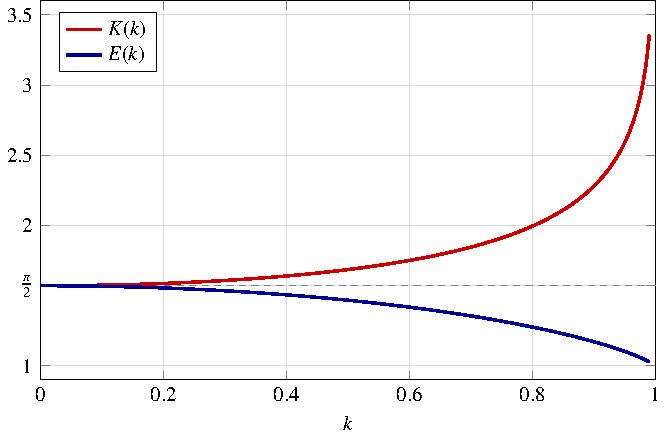
\includegraphics[width=0.72\textwidth]{papers/elliptisch/images/ke-plot.pdf}
	\caption{Die vollständigen elliptischen Integrale erster und
	zweiter Art.
	Beide starten bei $k=0$ im gemeinsamen Wert $\pi/2$.
	$E(k)$ fällt monoton auf $E(1) = 1$, während $K(k)$ monoton wächst
	und für $k \to 1$ logarithmisch divergiert.}
	\label{fig:elliptisch:keplot}
\end{figure}


\subsection{Der Ellipsenumfang mit $E(k)$
\label{elliptisch:subsection:ellipsenumfangE}}
Der Vergleich von \eqref{elliptisch:equation:legendreform} mit dem
Umfangsintegral \eqref{elliptisch:equation:umfang} zeigt, dass wir
die gesuchte Funktion bereits haben.
Das Integral zweiter Art in Legendre-Normalform ist Zeichen für
Zeichen der Ausdruck, der beim Ellipsenumfang stehen geblieben ist,
und damit gilt
\begin{equation}
U
=
4a\,E(k),
\qquad
k^2 = \frac{a^2-b^2}{a^2},
\qquad
a \ge b.
\label{elliptisch:equation:umfangE}
\end{equation}
Für den Kreis ist $k = 0$ und mit $E(0) = \pi/2$ folgt
$U = 4a\cdot\pi/2 = 2\pi a$.
Die Frage vom Anfang des Kapitels ist damit beantwortet, wenn auch
nicht durch eine elementare Formel, sondern durch eine eigens
definierte Funktion.
Dabei ist die Reihenfolge das Entscheidende.
Auch $\int dt/t$ war nicht darstellbar, solange es den Logarithmus
noch nicht gab, und erst seine Aufnahme in den Funktionsvorrat hat
das Integral lösbar gemacht.
Elementar ist also keine Eigenschaft eines Integrals an sich,
sondern eine Aussage über einen vorher festgelegten Vorrat.

\subsection{Unvollständige Integrale und Umkehrung
\label{elliptisch:subsection:unvollstaendig}}
Die vollständigen Integrale \eqref{elliptisch:equation:vollstaendig}
hängen nur von den Parametern $k$ und $n$ ab.
Funktionen der oberen Grenze entstehen, wenn wir sie variabel
machen.
\begin{definition}
\label{elliptisch:definition:unvollstaendig}
Die \emph{unvollständigen elliptischen Integrale} entstehen aus
den vollständigen, indem die obere Grenze $1$ durch die Variable
$x$ mit $0 \le x \le 1$ ersetzt wird,
\begin{equation}
\begin{aligned}
F(x,k)
&=
\int_0^x \frac{dt}{\sqrt{(1-t^2)(1-k^2t^2)}},
\\
E(x,k)
&=
\int_0^x \sqrt{\frac{1-k^2t^2}{1-t^2}}\,dt,
\\
\Pi(n,x,k)
&=
\int_0^x \frac{dt}{(1-nt^2)\sqrt{(1-t^2)(1-k^2t^2)}}.
\end{aligned}
\label{elliptisch:equation:unvollstaendig}
\end{equation}
\end{definition}
\index{elliptisches Integral!unvollstandiges@unvollständiges}%
Die Namen sind dieselben wie bei den vollständigen Integralen,
die Anzahl der Argumente unterscheidet die beiden Fassungen.
Zwei Spezialfälle halten wir fest.
An der oberen Grenze $x = 1$ wird aus dem unvollständigen
Integral wieder das vollständige, es ist $F(1,k) = K(k)$, und
entsprechend für die beiden anderen Arten.
Für $k = 0$ bleibt nur das Arcussinus-Integral stehen,
\begin{equation}
F(x,0)
=
E(x,0)
=
\int_0^x \frac{dt}{\sqrt{1-t^2}}
=
\arcsin x.
\label{elliptisch:equation:knullarcsin}
\end{equation}

Diese Zeile ist der Schlüssel zum nächsten Schritt.
Sie besagt, dass die Umkehrfunktion von $F(\,\cdot\,, 0)$ der
Sinus ist.
Dieselbe Geste, angewendet auf beliebiges $k$, liefert
\begin{equation}
\begin{aligned}
s
&=
\arcsin x
&\quad&\Leftrightarrow\quad&
x
&=
\sin s,
\\
u
&=
F(x,k)
&\quad&\Leftrightarrow\quad&
x
&=
\operatorname{sn}(u,k).
\end{aligned}
\label{elliptisch:equation:umkehrung}
\end{equation}
Die untere Zeile ist die Definition des
\emph{sinus amplitudinis} $\operatorname{sn}(u,k)$.
Weil der Integrand von $F$ positiv ist, wächst
$F(\,\cdot\,, k)$ streng monoton von $0$ auf $K(k)$, wenn $x$ das
Intervall $[0,1]$ durchläuft.
Die Umkehrfunktion existiert also und ist zunächst auf
$[0, K(k)]$ erklärt, definitionsgemäss gilt
$F(\operatorname{sn}(u,k), k) = u$.
\index{sn@$\operatorname{sn}(u,k)$}%

Den Namen erklärt die Legendre-Normalform.
Mit $x = \sin\varphi$ geht $u = F(x,k)$ in
\begin{equation}
u
=
\int_0^\varphi \frac{d\vartheta}{\sqrt{1-k^2\sin^2\vartheta}}
\label{elliptisch:equation:amplitude}
\end{equation}
über, und das Auflösen dieser Beziehung nach $\varphi$ liefert die
sogenannte \emph{Amplitude} $\varphi = \operatorname{am}(u,k)$.
Damit ist $\operatorname{sn}(u,k) = \sin\operatorname{am}(u,k)$,
der Sinus der Amplitude, also genau das, was der Name sagt.
\index{Amplitude}%

Die Bezeichnung \emph{sinus amplitudinis} stammt von Jacobi und
erklärt die Abkürzung $\operatorname{sn}$
\cite[Abschnitt~11.2]{elliptisch:mueller-spezielle}.
Der Schritt zur Umkehrung ist auch historisch der entscheidende.
Die elliptischen Integrale sind lange untersucht und tabelliert
worden, vor allem von Legendre.
Den \emph{Durchbruch} brachte erst ihre Umkehrung durch Abel und Jacobi,
mit der die elliptischen Funktionen entstanden sind.
1827 bewies Jacobi mit diesem Schritt seine allgemeine
Transformationsformel
\cite{elliptisch:wiki-elliptische-funktion}.
Was die neue Funktion mit dem Sinus gemeinsam hat und worin sie
sich von ihm unterscheidet, zeigt der nächste Abschnitt.

\subsection{Die geometrische Gestalt von sn, cn und dn
\label{elliptisch:subsection:geometrie}}
Was für den Sinus der Einheitskreis ist, ist für
$\operatorname{sn}$ eine Ellipse.
Der Einheitskreis fasst die Kreisfunktionen zusammen.
Sein Punkt, dessen Bogenlänge vom Punkt $(1,0)$ aus $u$ beträgt,
hat die Koordinaten $(\cos u, \sin u)$
(Abbildung~\ref{fig:elliptisch:snkonstruktion} links).
Auf der Ellipse mit den Halbachsen $a \ge 1$ und $1$,
\begin{equation}
\frac{x^2}{a^2} + y^2 = 1,
\label{elliptisch:equation:einheitsellipse}
\end{equation}
hängen Winkel, Bogenlänge und Koordinaten nicht mehr so einfach
zusammen.
Wir schreiben einen Punkt der Ellipse mit dem Hilfswinkel
$\varphi$ als
\begin{equation}
P
=
(a\cos\varphi, \sin\varphi)
\label{elliptisch:equation:ellipsenpunkt}
\end{equation}
und messen seine Lage durch den Parameter $u$ aus
\eqref{elliptisch:equation:amplitude}, sodass
$\varphi = \operatorname{am}(u,k)$ ist, mit dem Modul
$k = \sqrt{a^2-1}/a$.
Die drei jacobischen Funktionen sind die
Koordinatenverhältnisse dieses Punktes,
\begin{equation}
\operatorname{sn}(u,k) = y,
\qquad
\operatorname{cn}(u,k) = \frac{x}{a},
\qquad
\operatorname{dn}(u,k) = \frac{r}{a},
\qquad
r = \sqrt{x^2+y^2}.
\label{elliptisch:equation:geometrischedefinition}
\end{equation}
Die ersten beiden besagen
$\operatorname{sn}(u,k) = \sin\varphi = \sin\operatorname{am}(u,k)$
und $\operatorname{cn}(u,k) = \cos\varphi$, genau die Umkehrung
aus Abschnitt~\ref{elliptisch:subsection:unvollstaendig}.
Der gestrichelte Hilfskreis in
Abbildung~\ref{fig:elliptisch:snkonstruktion} trägt den Punkt
$Q = (\operatorname{cn}(u,k), \operatorname{sn}(u,k))$, an dem
sich der Winkel $\varphi$ ablesen lässt.
Für die dritte rechnet man $r^2 = a^2\cos^2\varphi + \sin^2\varphi$
nach und findet
\begin{equation}
\operatorname{dn}(u,k)^2
=
\frac{r^2}{a^2}
=
1 - k^2\sin^2\varphi
=
1 - k^2\operatorname{sn}(u,k)^2.
\label{elliptisch:equation:dngeometrie}
\end{equation}
\begin{figure}
	\centering
	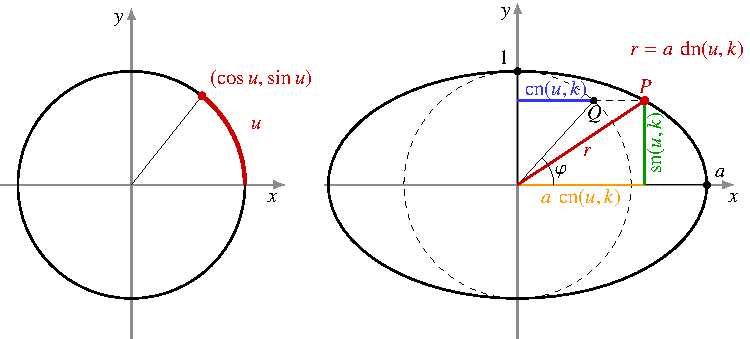
\includegraphics[width=\textwidth]{papers/elliptisch/images/sn-konstruktion.pdf}
	\caption{Links der Einheitskreis mit dem Punkt $(\cos u, \sin u)$
	zur Bogenlänge $u$.
	Rechts die Ellipse mit den Halbachsen $a = 1/k'$ und $1$ zum
	selben Parameter, hier $u = 0.9$ und $k = 0.8$.
	Die Punkte
	$Q = (\operatorname{cn}(u,k), \operatorname{sn}(u,k))$
	und
	$P = (a\operatorname{cn}(u,k), \operatorname{sn}(u,k))$
	liegen auf gleicher Höhe, der Abstand von $P$ zum Nullpunkt ist
	$r = a\operatorname{dn}(u,k)$.
	Nach \cite[Abschnitt~11.2.1]{elliptisch:mueller-spezielle} und
	\cite{elliptisch:schwalm}.}
	\label{fig:elliptisch:snkonstruktion}
\end{figure}


Der Parameter $u$ ist weder der Winkel $\varphi$ noch die
Bogenlänge der Ellipse.
Nur im Kreisfall $k = 0$ fallen alle drei zusammen.
Dann ist $a = 1$, die Ellipse wird zum Einheitskreis, und es gilt
$\operatorname{sn}(u,0) = \sin u$, $\operatorname{cn}(u,0) = \cos u$
und $\operatorname{dn}(u,0) = 1$, wie gewohnt.

Lässt man $\varphi$ von $0$ bis $2\pi$ laufen, durchläuft $P$ die
Ellipse einmal, und $u$ wächst von $0$ auf $4K(k)$.
Das Integral \eqref{elliptisch:equation:amplitude} legt $u$ zu
jedem Winkel $\varphi$ fest, und weil der Integrand positiv ist,
wächst $u$ mit $\varphi$ streng monoton über alle Grenzen.
Die Umkehrung $\varphi = \operatorname{am}(u,k)$ und damit
$\operatorname{sn}(u,k) = \sin\operatorname{am}(u,k)$ existieren
also für jedes reelle $u$, nicht mehr nur auf $[0, K(k)]$.
Auf das erste Viertel entfällt genau das Argument $u = K(k)$,
denn $\varphi = \pi/2$ bedeutet $y = 1$, und $F(1,k) = K(k)$.
Die Werte an den Viertelstellen sind damit
\begin{equation}
\begin{array}{c|ccccc}
u & 0 & K & 2K & 3K & 4K\\
\hline
\operatorname{sn}(u,k) & 0 & 1 & 0 & -1 & 0
\end{array}
\label{elliptisch:equation:snviertel}
\end{equation}
und es folgt die Periodizität
\begin{equation}
\operatorname{sn}(u + 4K(k), k)
=
\operatorname{sn}(u,k).
\label{elliptisch:equation:periode}
\end{equation}
Der Sinus hat die Periode $2\pi$, der sinus amplitudinis die
Periode $4K(k)$.
Beide Angaben vertragen sich, denn für $k = 0$ ist
$4K(0) = 2\pi$.
\index{Periodizitat@Periodizität}%

Der volle Funktionsverlauf zeigt sich aber erst in der komplexen
Ebene.
Dort besitzt $\operatorname{sn}$ neben der reellen Periode $4K$
noch die rein imaginäre Periode $2iK'$ mit $K' = K(k')$
\cite[Abschnitt~11.1.4, S.~307--308]{elliptisch:mueller-spezielle}.
Eine meromorphe Funktion mit zwei unabhängigen Perioden heisst
\emph{elliptische Funktion}.
Historisch waren die Umkehrfunktionen der elliptischen Integrale
die ersten bekannten Beispiele doppelt periodischer Funktionen,
weshalb die Bezeichnung von der Bogenlänge der Ellipse über die
Integrale zu diesen Funktionen wanderte
\cite{elliptisch:wiki-elliptische-funktion}.
\index{elliptische Funktion}%

\subsection{Der Werkzeugkasten
\label{elliptisch:subsection:werkzeugkasten}}
Die geometrische Deutung liefert fast von selbst die Rechenregeln,
mit denen in den Anwendungen gearbeitet wird.
Die Ellipsengleichung \eqref{elliptisch:equation:einheitsellipse}
und die Rechnung \eqref{elliptisch:equation:dngeometrie} schreiben
sich als die zwei Pythagoras-Identitäten
\begin{equation}
\operatorname{sn}^2(u,k) + \operatorname{cn}^2(u,k) = 1,
\qquad
\operatorname{dn}^2(u,k) + k^2\operatorname{sn}^2(u,k) = 1.
\label{elliptisch:equation:pythagoras}
\end{equation}

Die Ableitungen nach $u$ folgen aus der Wahl des Parameters.
Aus \eqref{elliptisch:equation:amplitude} liest man
\begin{equation}
\frac{du}{d\varphi}
=
\frac{1}{\sqrt{1-k^2\sin^2\varphi}}
=
\frac{1}{\operatorname{dn}(u,k)},
\qquad\text{also}\qquad
\frac{d\varphi}{du}
=
\operatorname{dn}(u,k)
\label{elliptisch:equation:dphidu}
\end{equation}
ab, und die Kettenregel ergibt
$\frac{d}{du}\operatorname{sn}(u,k)
= \cos\varphi \cdot \frac{d\varphi}{du}
= \operatorname{cn}(u,k)\,\operatorname{dn}(u,k)$.
Dieselbe Rechnung für die beiden anderen Funktionen liefert
zusammen
\begin{equation}
\begin{aligned}
\frac{d}{du}\operatorname{sn}(u,k) &= \operatorname{cn}(u,k)\,\operatorname{dn}(u,k),\\
\frac{d}{du}\operatorname{cn}(u,k) &= -\operatorname{sn}(u,k)\,\operatorname{dn}(u,k),\\
\frac{d}{du}\operatorname{dn}(u,k) &= -k^2\operatorname{sn}(u,k)\,\operatorname{cn}(u,k),
\end{aligned}
\label{elliptisch:equation:ableitungen}
\end{equation}
siehe \cite[Satz~11.11]{elliptisch:mueller-spezielle}.
Quadrieren der ersten Zeile und Einsetzen der Identitäten
\eqref{elliptisch:equation:pythagoras} ergibt die
Differentialgleichung
\begin{equation}
\operatorname{sn}'(u,k)^2
=
\bigl(1-\operatorname{sn}^2(u,k)\bigr)
\bigl(1-k^2\operatorname{sn}^2(u,k)\bigr).
\label{elliptisch:equation:sndgl}
\end{equation}
Sie hat die Signatur
\begin{equation}
(y')^2
=
\alpha y^4 + \beta y^2 + \gamma,
\label{elliptisch:equation:signatur}
\end{equation}
ein Polynom vierten Grades in $y$ ohne ungerade Potenzen.
Die Funktionen $\operatorname{cn}$ und $\operatorname{dn}$ erfüllen
Gleichungen derselben Signatur mit anderen Koeffizienten
\cite[Abschnitt~11.2.2]{elliptisch:mueller-spezielle}.
Genau diese Signatur wird in den Anwendungen von
Abschnitt~\ref{elliptisch:section:anwendungen} wieder auftauchen.
Führt die Physik auf eine Gleichung der Form
\eqref{elliptisch:equation:signatur}, ist die Lösung eine
jacobische Funktion.

Die Grenzfälle des Moduls geben die Brücke zu Bekanntem.
Für $k = 0$ wird $\operatorname{sn}$ zu $\sin$, $\operatorname{cn}$
zu $\cos$ und $\operatorname{dn}$ konstant $1$, wie im
vorangegangenen Abschnitt gesehen.
Für $k = 1$ wird \eqref{elliptisch:equation:sndgl} zu
$y' = 1 - y^2$ mit der Lösung $\operatorname{sn}(u,1) = \tanh u$,
und entsprechend
$\operatorname{cn}(u,1) = \operatorname{dn}(u,1)
= \operatorname{sech} u$
\cite[Abschnitt~11.2.1]{elliptisch:mueller-spezielle}.
Zwischen den Kreisfunktionen und den hyperbolischen Funktionen
liegt also eine ganze Schar von Funktionen, parametrisiert durch
$k$.

Zur Notation sei noch erwähnt, dass Kehrwerte und Quotienten der
drei Grundfunktionen eigene zweibuchstabige Namen tragen, etwa
$\operatorname{sc} = \operatorname{sn}/\operatorname{cn}$,
insgesamt zwölf Funktionen nach Glaisher
\cite[Abschnitt~11.2, Tabelle~11.3]{elliptisch:mueller-spezielle}.
\index{Glaisher-Notation}%

%
% anwendungen.tex -- Anwendungen der elliptischen Funktionen
%
% (c) 2026 Baris Catan, OST Ostschweizer Fachhochschule
%
% !TEX root = ../../buch.tex
% !TEX encoding = UTF-8
%
\section{Anwendungen
\label{elliptisch:section:anwendungen}}
\kopfrechts{Anwendungen}

Mit dem Werkzeugkasten von
Abschnitt~\ref{elliptisch:subsection:werkzeugkasten} ist klar, woran
man eine jacobische Lösung erkennt.
Führt ein Problem auf die Differentialgleichung
\eqref{elliptisch:equation:signatur}, also das Quadrat der Ableitung
gleich einem Polynom vierten Grades, dann ist die Lösung eine
jacobische Funktion.
In diesem Abschnitt taucht diese Signatur dreimal auf.
Wir beginnen bei der Kurve, an der die Theorie historisch ihren
Anfang genommen hat, und kommen danach zu zwei physikalischen
Problemen, einem rotierenden Seil und einem Pendel.

\subsection{Die Lemniskate
\label{elliptisch:subsection:lemniskate}}
\index{Lemniskate}%
Die \emph{Lemniskate von Bernoulli} ist die Kurve vierten Grades
mit der Gleichung
\begin{equation}
(X^2+Y^2)^2 = 2a^2\,(X^2-Y^2).
\label{elliptisch:equation:lemniskate}
\end{equation}
Wir verwenden die Normierung $a = 1/\sqrt{2}$, in der die Scheitel
bei $(\pm 1, 0)$ liegen (Abbildung~\ref{fig:elliptisch:lemniskate}).
\begin{figure}
	\centering
	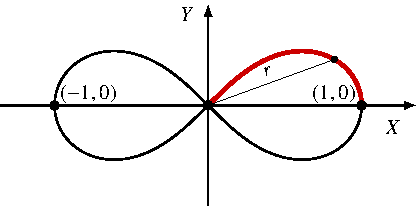
\includegraphics[width=0.56\textwidth]{papers/elliptisch/images/lemniskate.pdf}
	\caption{Die Lemniskate von Bernoulli mit $a = 1/\sqrt{2}$ und
	den Scheiteln bei $(\pm 1, 0)$.
	Hervorgehoben ist der Bogen vom Nullpunkt bis zum Scheitel
	$(1,0)$, seine Länge ist $\varpi/2$.}
	\label{fig:elliptisch:lemniskate}
\end{figure}
%
In Polarkoordinaten schreibt sie sich als $r^2 = \cos 2\varphi$.
Das Bogenelement in Polarkoordinaten ist
$ds^2 = dr^2 + r^2\,d\varphi^2$ und Differenzieren der
Kurvengleichung ergibt $2r\,dr = -2\sin 2\varphi\,d\varphi$.
Damit lässt sich $\varphi$ eliminieren,
\begin{equation}
r^2\,d\varphi^2
=
\frac{r^4}{\sin^2 2\varphi}\,dr^2
=
\frac{r^4}{1-r^4}\,dr^2,
\label{elliptisch:equation:phielimination}
\end{equation}
denn es ist $\sin^2 2\varphi = 1 - \cos^2 2\varphi = 1 - r^4$.
Somit bleibt im Bogenelement nur noch der Radius,
\begin{equation}
ds
=
\sqrt{1 + \frac{r^4}{1-r^4}}\,dr
=
\frac{dr}{\sqrt{1-r^4}}.
\label{elliptisch:equation:bogenelementr}
\end{equation}
Die Bogenlänge vom Nullpunkt bis zum Punkt mit Radius $r$ ist damit
\begin{equation}
s(r)
=
\int_0^r \frac{dt}{\sqrt{1-t^4}}.
\label{elliptisch:equation:lemniskatebogen}
\end{equation}
Unter der Wurzel steht mit $1-t^4 = (1-t^2)(1+t^2)$ wieder ein
Polynom vierten Grades ohne mehrfache Nullstellen, das Integral
fällt also unter die Definition
\eqref{elliptisch:equation:definition}.
Der direkte Vergleich mit der Normalform
\eqref{elliptisch:equation:normalformen} liefert formal
$k^2 = -1$, ausserhalb des Bereichs von
Satz~\ref{elliptisch:satz:nichtelementar}.
Wie Gleichung \eqref{elliptisch:equation:sljacobi} weiter unten
zeigt, gehört das Integral nach einer Substitution zum Modul
$k = 1/\sqrt{2}$, und weil diese Substitution algebraisch ist,
überträgt sich der Satz, eine elementare Stammfunktion existiert
nicht.
Der Kontrast zum Kreis wiederholt sich.
Das Integral $\int_0^r dt/\sqrt{1-t^2} = \arcsin r$ bleibt
elementar, das Bogenlängenintegral der Lemniskate nicht.

Wie in \eqref{elliptisch:equation:umkehrung} kehren wir um.
Die Umkehrfunktion $r = \operatorname{sl}(s)$ heisst
\emph{lemniskatischer Sinus}.
\index{lemniskatischer Sinus}%
Leitet man \eqref{elliptisch:equation:lemniskatebogen} nach $s$ ab,
folgt $(\operatorname{sl}')^2 = 1 - \operatorname{sl}^4$, wieder die
Signatur \eqref{elliptisch:equation:signatur} aus dem
Werkzeugkasten.
Der Bogen vom Nullpunkt bis zum Scheitel $(1,0)$ hat die Länge
$\varpi/2$, wobei
\begin{equation}
\varpi
=
2\int_0^1 \frac{dt}{\sqrt{1-t^4}}
=
2.6220575542\ldots
\label{elliptisch:equation:varpi}
\end{equation}
die Länge des rechten Blattes ist, die sogenannte
\emph{lemniskatische Konstante}.
\index{lemniskatische Konstante}%
Die Funktion $\operatorname{sl}$ ist $2\varpi$-periodisch, und was
für den Sinus die Zahl $\pi$ ist, ist für ihn $\varpi$.
Historisch war der lemniskatische Sinus die erste elliptische
Funktion überhaupt.
Gauss hat sie 1797 als Neunzehnjähriger in seinem mathematischen
Tagebuch untersucht, zu Lebzeiten aber nichts davon veröffentlicht
\cite{elliptisch:almkvist-berndt} und
\cite[Abschnitt~11.3]{elliptisch:mueller-spezielle}.
Erst dreissig Jahre später wurde derselbe Umkehrschritt von Abel
und Jacobi in voller Allgemeinheit vollzogen
(Abschnitt~\ref{elliptisch:subsection:unvollstaendig}).

Die Verbindung zu den jacobischen Funktionen gewinnt man aus der
Bogenlängenparametrisierung der Lemniskate.
Aus ihr folgt
\begin{equation}
\operatorname{sl}(s)
=
\operatorname{cn}\biggl(
\sqrt{2}\,\Bigl(\frac{\varpi}{2}-s\Bigr),\,
\frac{1}{\sqrt{2}}
\biggr),
\label{elliptisch:equation:sljacobi}
\end{equation}
der lemniskatische Sinus ist also bis auf Skalierung und
Verschiebung des Arguments die Funktion $\operatorname{cn}$ zum
Modul $k = 1/\sqrt{2}$
\cite[Abschnitt~11.3]{elliptisch:mueller-spezielle}.
Insbesondere ist $\varpi = \sqrt{2}\,K(1/\sqrt{2})$, ganz analog zu
$\pi = 2K(0)$ in \eqref{elliptisch:equation:randnull}.

\subsection{Das Troposkein
\label{elliptisch:subsection:troposkein}}
\index{Troposkein}%
\index{Springseil}%
Eine Schnur hängt zwischen zwei Punkten $A$ und $B$.
Unter der Schwerkraft nimmt sie die Kettenlinie an, einen
hyperbolischen Kosinus, ein durch und durch elementares Resultat.
Lassen wir dieselbe Schnur stattdessen mit der
Winkelgeschwindigkeit $\omega$ um die Verbindungsachse von $A$
und $B$ rotieren und vernachlässigen die Schwerkraft, entsteht
eine neue Gleichgewichtsform.
Sie heisst \emph{Troposkein} oder Springseilkurve
\cite{elliptisch:skipping-rope}.
Abbildung~\ref{fig:elliptisch:troposkein} zeigt das Profil der
rotierenden Schnur zwischen $A$ und $B$.
\begin{figure}
	\centering
	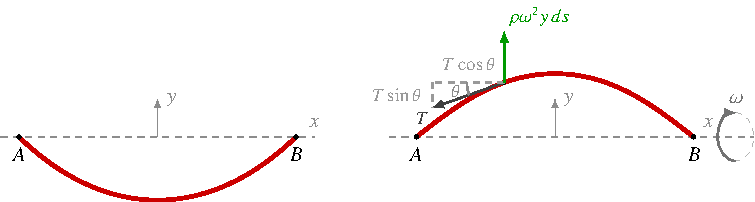
\includegraphics[width=\textwidth]{papers/elliptisch/images/troposkein.pdf}
	\caption{Links die hängende Schnur zwischen $A$ und $B$ bei
	$x = \pm l$, die Kettenlinie
	$y(x) = d\,(\cosh(x/d) - \cosh(l/d))$.
	Rechts rotierend um $AB$, das Troposkein
	\mbox{$y(x) = a\operatorname{sn}((x+l)/c, k)$}, mit
	Zentrifugalkraft $\rho\omega^2y\,ds$ und Seilspannung $T$ am
	Element mit Winkel $\theta$.}
	\label{fig:elliptisch:troposkein}
\end{figure}
%

Wir bezeichnen mit $y(x)$ den Abstand eines Seilpunktes von der
Drehachse, mit $\theta$ den Winkel der Seiltangente gegen die
Achse, mit $\rho$ die Linienmassendichte und mit $T$ die
Seilspannung (Abbildung~\ref{fig:elliptisch:troposkein}, rechts).
Auf ein Element der Länge $ds$ wirkt die Zentrifugalkraft
$\rho\omega^2 y\,ds$ radial nach aussen.
Im Gleichgewicht ist die axiale Komponente der Spannung konstant,
\begin{equation}
T\cos\theta = T_0,
\label{elliptisch:equation:troposkeinaxial}
\end{equation}
und die Änderung ihrer Querkomponente entlang der Bogenlänge trägt
die Zentrifugalkraft,
\begin{equation}
\frac{d(T\sin\theta)}{ds}
=
-\rho\omega^2 y.
\label{elliptisch:equation:troposkeinradial}
\end{equation}
Aus \eqref{elliptisch:equation:troposkeinaxial} folgt durch
Differenzieren die Beziehung
$dT/ds = \sin\theta \cdot d(T\sin\theta)/ds$.
Multipliziert man \eqref{elliptisch:equation:troposkeinradial} mit
$\sin\theta$, steht damit
\begin{equation}
\frac{dT}{ds}
=
-\rho\omega^2 y\,\frac{dy}{ds},
\label{elliptisch:equation:troposkeinintegration}
\end{equation}
und die Integration nach $y$ liefert
die Spannung als Funktion des Abstandes,
\begin{equation}
T(y)
=
T_0 + \frac{\rho\omega^2}{2}\,\bigl(a^2 - y^2\bigr),
\label{elliptisch:equation:troposkeinspannung}
\end{equation}
wobei $a$ der grösste Achsabstand ist, also der Scheitel der Kurve,
an dem $\theta = 0$ und $T = T_0$ gilt.
Die Spannung ist folglich in der Mitte am kleinsten und an den
Endpunkten am grössten.

Die Ableitung der Kurve ist $y' = \tan\theta$, und mit
$\tan^2\theta = (T/T_0)^2 - 1$ wird aus
\eqref{elliptisch:equation:troposkeinspannung} nach Quadrieren und
Zusammenfassen der Konstanten
\begin{equation}
(y')^2
=
\frac{1}{c^2}\,\bigl(a^2 - y^2\bigr)
\biggl(1 - \frac{b^2 y^2}{a^4}\biggr)
\label{elliptisch:equation:troposkein}
\end{equation}
mit zwei Konstanten $b \le a$ und $c$, die sich aus den
physikalischen Grössen und den Randbedingungen bestimmen.
Rechts steht ein Polynom vierten Grades in $y$, genau die Signatur
\eqref{elliptisch:equation:signatur} aus dem Werkzeugkasten.
Die Lösung muss daher eine jacobische Funktion sein.
Wir machen den Ansatz, mit $x$ von der Mitte aus gemessen und
$A$ bei $x = -l$,
\begin{equation}
y(x)
=
a\,\operatorname{sn}\Bigl(\frac{x+l}{c}, k\Bigr),
\qquad
k = \frac{b}{a},
\label{elliptisch:equation:troposkeinloesung}
\end{equation}
und setzen ihn zur Probe ein.
Nach \eqref{elliptisch:equation:sndgl} ist
$(y')^2 = (a^2/c^2)\,\operatorname{cn}^2\operatorname{dn}^2
= (1/c^2)\,(a^2-y^2)\,(1 - k^2y^2/a^2)$,
was mit $k = b/a$ genau die rechte Seite von
\eqref{elliptisch:equation:troposkein} ergibt.
Die Randbedingungen legen die Konstanten fest.
Das Seil geht bei $A$ und $B$ durch $y = 0$ und erreicht seine
grösste Auslenkung in der Mitte, also ist $l = c\,K(k)$, und die
vorgegebene Seillänge liefert die zweite Bedingung an $b$ und $c$.

Welche Form das Seil annimmt, bestimmt der Modul, und der kommt
aus der Physik.
Setzt man \eqref{elliptisch:equation:troposkeinspannung} in
$(y')^2 = (T/T_0)^2 - 1$ ein und vergleicht mit
\eqref{elliptisch:equation:troposkein}, liest man
\begin{equation}
k^2
=
\frac{b^2}{a^2}
=
\frac{a^2}{a^2 + 4T_0/(\rho\omega^2)}
\label{elliptisch:equation:troposkeinmodul}
\end{equation}
ab.
Schnelle Rotation bei schwacher Spannung treibt $k$ gegen $1$,
starke Spannung gegen $0$.

Damit stellt sich heraus, dass das Auge uns hier täuscht.
Die Springseilkurve sieht aus wie eine Sinushalbwelle, ist aber ein
jacobischer Sinus als Funktion des \emph{Ortes}.
Was die Form verändert, ist allein der Modul.
Nach den Grenzfällen aus
Abschnitt~\ref{elliptisch:subsection:werkzeugkasten} ist
$\operatorname{sn}$ für $k = 0$ der gewöhnliche Sinus, während die
Halbwelle für $k \to 1$ ein Plateau und steile Flanken bekommt.
Mit \eqref{elliptisch:equation:troposkeinmodul} wird dieses Plateau
also breiter, je schneller das Seil rotiert.
Dieselbe Signatur \eqref{elliptisch:equation:signatur} wird uns
in Abschnitt~\ref{elliptisch:subsection:pendel} wieder begegnen,
dort mit der Zeit als unabhängiger Variable.

Die Form hat auch eine technische Seite.
Die Schaufeln des Darrieus-Rotors werden im Troposkein-Profil
gebaut, weil die Zentrifugalkraft ein Seil in dieser Form nur auf
Zug belastet und nicht auf Biegung
\cite{elliptisch:wiki-darrieus}.
\index{Darrieus-Rotor}%
Dessen Achse steht senkrecht, und damit wirkt die Schwerkraft
längs der Achse.
Sie geht in die axiale Bilanz ein, aus
\eqref{elliptisch:equation:troposkeinaxial} wird
$d(T\cos\theta)/ds = \rho g$, und das Troposkein ist nur noch eine
Näherung.
Bei Betriebsdrehzahl ist $\omega^2 y$ jedoch um Grössenordnungen
grösser als $g$, sodass die Abweichung klein bleibt.
\begin{figure}
	\centering
	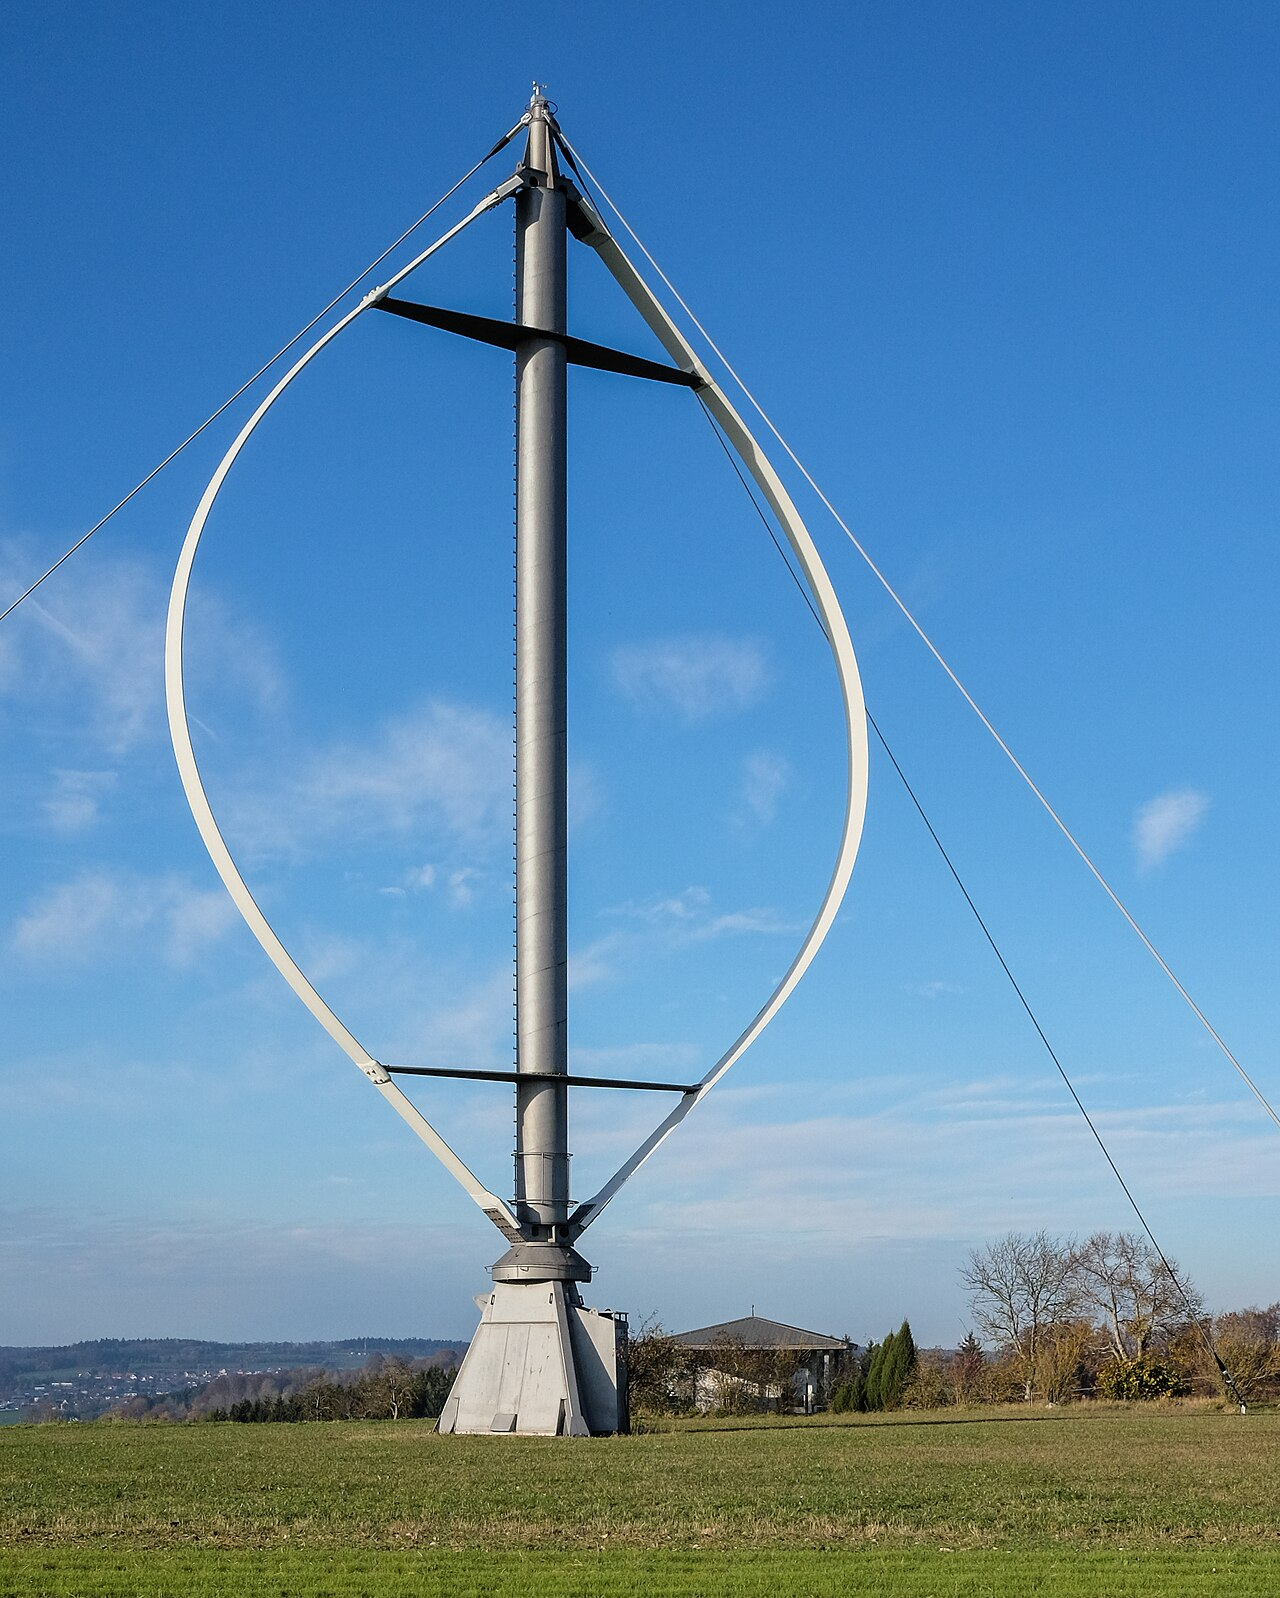
\includegraphics[width=0.5\textwidth]{papers/elliptisch/images/darrieus-rotor.jpg}
	\caption{Ein Darrieus-Rotor mit zwei Schaufeln im
	Troposkein-Profil.
	Bild: \cite{elliptisch:darrieus-bild}.}
	\label{fig:elliptisch:darrieus}
\end{figure}


\subsection{Das Pendel
\label{elliptisch:subsection:pendel}}
Wie am Ende von Abschnitt~\ref{elliptisch:subsection:troposkein}
angekündigt, begegnet uns die Signatur
\eqref{elliptisch:equation:signatur} jetzt mit der Zeit als
unabhängiger Variable.
Ein Massepunkt der Masse $m$ hängt an einem masselosen Stab der
Länge $l$, und $\vartheta$ sei der Auslenkwinkel gegen das Lot
(Abbildung~\ref{fig:elliptisch:pendel}, links).
\begin{figure}
	\centering
	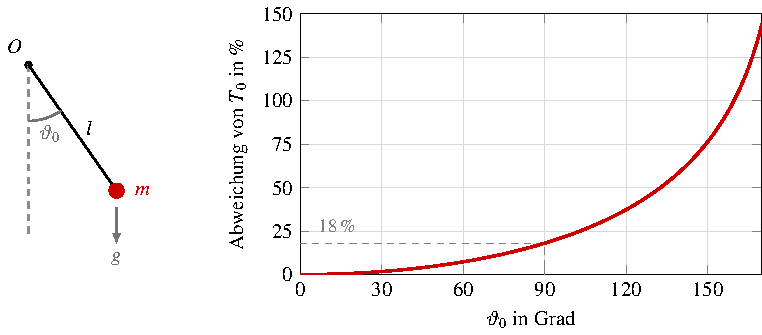
\includegraphics[width=\textwidth]{papers/elliptisch/images/pendel.pdf}
	\caption{Links das mathematische Pendel der Länge $l$ mit der
	Amplitude $\vartheta_0$.
	Rechts die Abweichung der exakten Schwingungsdauer
	$T = 4\sqrt{l/g}\,K(k)$ von der Kleinwinkelnäherung
	$T_0 = 2\pi\sqrt{l/g}$ in Prozent, aufgetragen über
	$\vartheta_0$.
	Bei $90^\circ$ sind es $18\,\%$.}
	\label{fig:elliptisch:pendel}
\end{figure}
%
Die Bewegungsgleichung des Pendels ist
\begin{equation}
\ddot{\vartheta} = -\frac{g}{l}\,\sin\vartheta.
\label{elliptisch:equation:pendelbewegung}
\end{equation}
Wir verzichten auf die Kleinwinkelnäherung
\index{Kleinwinkelnäherung}%
$\sin\vartheta \approx \vartheta$ und rechnen exakt.

Die Multiplikation von \eqref{elliptisch:equation:pendelbewegung}
mit $\dot\vartheta$ und Integration über die Zeit liefert die
Energieerhaltung, ein erstes Integral der Bewegungsgleichung.
Startet das Pendel aus der Ruhe bei der Amplitude $\vartheta_0$, so
ist
\begin{equation}
\frac{1}{2}\,ml^2\dot\vartheta^2 + mgl\,(1-\cos\vartheta)
=
mgl\,(1-\cos\vartheta_0).
\label{elliptisch:equation:pendelenergie}
\end{equation}
Mit $1-\cos\vartheta = 2\sin^2(\vartheta/2)$ folgt
$\dot\vartheta^2 = (4g/l)\,\bigl(\sin^2(\vartheta_0/2)
-\sin^2(\vartheta/2)\bigr)$, und die Substitution
$y = \sin(\vartheta/2)$ mit
$\dot y^2 = \frac14\,(1-y^2)\,\dot\vartheta^2$ ergibt
\begin{equation}
\dot y^2
=
\frac{g}{l}\,(1-y^2)\,\bigl(y_0^2-y^2\bigr),
\qquad
y_0 = \sin\frac{\vartheta_0}{2}.
\label{elliptisch:equation:pendeldgl}
\end{equation}
Rechts steht wieder die Signatur
\eqref{elliptisch:equation:signatur}.
Die Normierung $z = y/y_0$ auf die Amplitude und
$u = \sqrt{g/l}\,t$ auf die Zeit macht daraus
\begin{equation}
\biggl(\frac{dz}{du}\biggr)^2
=
(1-z^2)\,\bigl(1-y_0^2 z^2\bigr),
\label{elliptisch:equation:pendelnormiert}
\end{equation}
exakt die Gleichung \eqref{elliptisch:equation:sndgl} des
jacobischen Sinus.
Damit ist $z = \operatorname{sn}(u,k)$ mit dem Modul
$k = y_0 = \sin(\vartheta_0/2)$, der die Amplitude misst.
Die Energie ist $E = 2mgl\,k^2$
\cite[Abschnitt~11.2.3]{elliptisch:mueller-spezielle}.

Jetzt machen wir die beiden Substitutionen rückgängig.
Aus $z = y/y_0$ und $k = y_0$ wird
$y = y_0 z = k\,\operatorname{sn}(u,k)$, und mit
$y = \sin(\vartheta/2)$ sowie $u = \sqrt{g/l}\,t$ ist
\begin{equation}
\sin\frac{\vartheta}{2}
=
k\,\operatorname{sn}\bigl(\sqrt{g/l}\;t,\,k\bigr),
\qquad\text{also}\qquad
\vartheta(t)
=
2\arcsin\Bigl(k\,\operatorname{sn}\bigl(\sqrt{g/l}\;t,\,k\bigr)\Bigr).
\label{elliptisch:equation:pendelloesung}
\end{equation}
Eine volle Schwingung durchläuft in $u$ die Periode $4K(k)$.
Gesucht ist aber die Periode in der Zeit und nicht in $u$.
Wegen $t = u\sqrt{l/g}$ wird daraus die Schwingungsdauer
\begin{equation}
T = 4\,\sqrt{\frac{l}{g}}\;K(k).
\label{elliptisch:equation:pendelperiode}
\end{equation}

Für kleine Amplituden geht $k$ gegen $0$, und mit $K(0) = \pi/2$
aus \eqref{elliptisch:equation:randnull} kommt
$T \to 2\pi\sqrt{l/g}$ heraus, die Kleinwinkelnäherung kehrt als
Grenzfall zurück.
Bei $\vartheta_0 = 90^\circ$ ist die Periode bereits um $18\,\%$
länger als die Kleinwinkelformel, bei $\vartheta_0 = 179^\circ$
um den Faktor $3.9$
(Abbildung~\ref{fig:elliptisch:pendel}, rechts).
Für $k \to 1$, also $\vartheta_0 \to \pi$, divergiert $K(k)$
logarithmisch wie in \eqref{elliptisch:equation:kasymptotik}, und
die Schwingungsdauer wächst über alle Grenzen, das Pendel erreicht
den oberen Scheitelpunkt asymptotisch nie.

%
% schluss.tex -- Rueckblick und Ausblick
%
% (c) 2026 Baris Catan, OST Ostschweizer Fachhochschule
%
% !TEX root = ../../buch.tex
% !TEX encoding = UTF-8
%
\section{Eine folgenreiche Antwort
\label{elliptisch:section:schluss}}
\kopfrechts{Eine folgenreiche Antwort}

Die harmlose Frage nach dem Umfang der Ellipse hat mehrere grosse
Gebiete der Mathematik hervorgebracht.
Die Frage nach der elementaren Lösbarkeit ist zunächst in der
Analysis formuliert und mit dem Satz von Liouville
\eqref{elliptisch:equation:liouville} in der Algebra entschieden
worden.

Untersucht haben wir die Grenze an Integralen des Typs
$R\bigl(x,\sqrt{p(x)}\bigr)$ und daran, wo ihre elementare
Lösbarkeit endet.
Über den Reduktionssatz~\ref{elliptisch:satz:reduktion} sind daraus
die drei vollständigen Integrale $K$, $E$ und $\Pi$ entstanden.
Lässt man die obere Grenze variieren, so werden daraus die
unvollständigen Integrale, die historisch unhandlich blieben.
Den Durchbruch brachte erst ihre geschickte Umkehrung, aus der die
jacobischen elliptischen Funktionen $\operatorname{sn}$,
$\operatorname{cn}$ und $\operatorname{dn}$ hervorgegangen sind.
Sie erfüllen Identitäten und Additionstheoreme wie die bekannten
Kreisfunktionen, haben einfache Ableitungen und sind Lösungen der
Differentialgleichungen aus
Abschnitt~\ref{elliptisch:section:anwendungen}.
Nur kurz eingegangen sind wir auf ihre doppelte Periodizität, die
sich erst in der komplexen Ebene zeigt, wo diese Funktionen auch
vollständig zu verstehen sind.
Von dort aus haben die Theorie der riemannschen Flächen, die
Modulformen und die Arithmetik der elliptischen Kurven ihren
Aufschwung genommen, deren Anwendungen heute bis in die
Kryptographie reichen.
\index{riemannsche Flache@riemannsche Fläche}%
\index{Modulform}%

Dieses Kapitel deckt nur einen Bruchteil dessen ab, was aus dieser
Richtung gewachsen ist, von den Anwendungen bis zu ganzen neuen
Zweigen der Mathematik.
Was am Anfang wie eine Grenze der Analysis aussah, erwies sich als
Eingang zu einer eigenen Theorie.


\printbibliography[heading=subbibliography]
\end{refsection}
